\documentclass[a4paper, 12pt]{extarticle}

\usepackage{xecyr}
\usepackage{color}
\usepackage{float}
\usepackage{fontenc}
\usepackage{amsmath}
\usepackage{xltxtra}
\usepackage{graphicx}
\usepackage{csquotes}
\usepackage{listings}
\usepackage{longtable}
\usepackage{indentfirst}
\usepackage{unicode-math}
\usepackage[english, russian]{babel}
\usepackage[width=1.2\textwidth]{caption}

\usepackage{tikz}
\usetikzlibrary{arrows, shapes, positioning, shadows, trees}
\tikzset{
  basic/.style  = {draw, text width=4cm, drop shadow, font=\sffamily, rectangle},
  root/.style   = {basic, rounded corners=2pt, thin, align=center, fill=gray!1},
  level 1/.style = {basic, rounded corners=2pt, thin, align=center, fill=gray!1,
                    sibling distance=55mm, level distance=50pt,
                    edge from parent/.style={->,draw,fill=black},
                    >=latex},
  level 2/.style = {basic, rounded corners=2pt, thin, align=center, fill=gray!1,
                    sibling distance=55mm, level distance=50pt,
                    edge from parent/.style={->,draw,fill=black},
                    >=latex},
  level 3/.style = {basic, rounded corners=2pt, thin, align=center, fill=gray!1,
                    sibling distance=55mm, level distance=75pt,
                    edge from parent/.style={->,draw,fill=black},
                    >=latex, text width=5cm},
  level 4/.style = {basic, rounded corners=2pt, thin, align=center, fill=gray!1,
                    sibling distance=40mm, level distance=50pt,
                    edge from parent/.style={->,draw,fill=black},
                    >=latex, text width=3cm},
}


\usepackage{titlesec}
\titleformat{\section}
  {\normalfont\fontsize{14}{15}\bfseries}{\thesection}{5pt}{}
\titleformat{\subsection}
  {\normalfont\fontsize{14}{15}\bfseries}{\thesubsection}{5pt}{}
\titleformat{\subsubsection}
  {\normalfont\fontsize{14}{15}\bfseries}{\thesubsubsection}{5pt}{}

\usepackage{fontspec}
\defaultfontfeatures{Ligatures=TeX}
\setmainfont[Ligatures=TeX]{Times New Roman}

\usepackage[a4paper,margin=1in,heightrounded]{geometry}
\geometry{left=3cm}
\geometry{right=1.5cm}
\geometry{top=2cm}
\geometry{bottom=2cm}

\usepackage{expl3}
\ExplSyntaxOn
\cs_new_eq:NN \Repeat \prg_replicate:nn
\ExplSyntaxOff

\usepackage[maxnames=5,
				movenames=false,
				backend=bibtex,
        %backend=biber,
				%style=gost-numeric,
        sorting=none,
				autolang=other]{biblatex}
\addbibresource{bibliography.bib}


% Sections style redefinition
\renewcommand{\thesection}
  {\thepart\arabic{section}.}
\renewcommand{\thesubsection}
  {\thepart\arabic{section}.\arabic{subsection}.}
\renewcommand{\thesubsubsection}
  {\thepart\arabic{section}.\arabic{subsection}.\arabic{subsubsection}.}

% Equations, fugures, tables numbering style redefinition
\renewcommand{\theequation}
  {\thesection\arabic{equation}}
\renewcommand{\thefigure}
  {\thesection\arabic{figure}}
\renewcommand{\thetable}
  {\thesection\arabic{table}}

% Enum style redefinition
\renewcommand{\labelenumii}
  {\labelenumi\arabic{enumii}.}
\renewcommand{\labelenumiii}
  {\labelenumii\arabic{enumiii}.}

% Enlarge table row height
\renewcommand{\arraystretch}{1.2}

% Font to inline code highlighting
% Consolas must be installed!!!
\newfontfamily{\codefont}[Scale=0.9]{Consolas}
\newfontfamily{\listingsfont}[Scale=1.0]{Consolas}

% Define default style for codelisitngs
\definecolor{codegreen}{rgb}{0.00, 0.50, 0.00}
\definecolor{codegray} {rgb}{0.50, 0.50, 0.50}
\definecolor{codenumb} {rgb}{0.00, 0.00, 1.00}
\definecolor{codeblue} {rgb}{0.00, 0.43, 0.13}
\definecolor{codebrick}{rgb}{0.64, 0.08, 0.08}
\lstset{
  backgroundcolor=\color{white},
  basicstyle=\fontsize{10}{12}\selectfont\listingsfont,
  breakatwhitespace=false,
  breaklines=true,
  captionpos=b,
  commentstyle=\color{codegreen},
  frame=l,
  keepspaces=true,
  keywordstyle=\color{codeblue},
  language=C++,
  numbers=left,
  numbersep=8pt,
  numberstyle=\tiny\color{codegray},
  rulecolor=\color{black},
  showspaces=false,
  showstringspaces=false,
  showtabs=false,
  stepnumber=1,
  stringstyle=\color{codebrick},
  tabsize=2,
  title=\lstname
}

% Listing numbering style redefinition
\renewcommand{\lstlistingname}{Листинг}
\AtBeginDocument{
  \renewcommand{\thelstlisting}{\thesection\arabic{lstlisting}}
}

\DeclareMathOperator*{\argmax}{arg\,max}
\DeclareMathOperator*{\argmin}{arg\,min}
\DeclareMathOperator{\sign}{sign}

\begin{document}

\begingroup
\fontsize{14pt}{17pt}\selectfont
\begin{titlepage}

\begin{center}
МИНИСТЕРСТВО ОБРАЗОВАНИЯ И НАУКИ РОССИЙСКОЙ ФЕДЕРАЦИИ \\*
Федеральное   государственное  автономное  образовательное  учреждение \\*
высшего образования \\*
\textbf{<<Национальный исследовательский \\*
Нижегородский государственный университет им. Н.И. Лобачевского>> \\*
(ННГУ)}
\end{center}

\vspace{12pt}

\begin{center}
\textbf{Институт информационных технологий, математики и механики}
\end{center}

\begin{center}
\textbf{Кафедра: Математического обеспечения и суперкомпьютерных технологий}
\end{center}

\vspace{25pt}
\begin{center}
Направление подготовки: «Прикладная математика и информатика» \\*
Магистерская программа: «Системное программирование»
\end{center}
\vspace{30pt}

\begin{center}
\fontsize{18pt}{0pt}\textbf{ОТЧЁТ} \\*
по научно-исследоваетльской практике
\end{center}
\begin{center}
на тему: \\*
\fontsize{16pt}{0pt}\textbf{Разработка эффективных структурх хранения данных для алгоритмов глобальной оптимизации}
\end{center}

\vspace{53pt}

\begin{flushright}
\textbf{Выполнил}: студент группы 381503м2 \\*
\Repeat{17}{\_} Соврасов В.В. \\*
Подпись \Repeat{32}{\ } \\*

\textbf{Научный руководитель}: \Repeat{19}{\ } \\*
доцент, к.ф.м.н. \Repeat{34}{\ } \\*
\Repeat{17}{\_} Баркалов К.А. \\*
Подпись \Repeat{32}{\ }
\end{flushright}

\vspace{\fill}

\begin{center}
Нижний Новгород \\*
2016
\end{center}

\end{titlepage}
 % Link to main page
\endgroup

\begingroup
\fontsize{12pt}{20pt}\selectfont

\newpage
\thispagestyle{empty}
\tableofcontents

\newpage
\setcounter{page}{1}
\section{Введение}
//здесь про важность задач глобаьной оптимизации
Задачи глобальной оптимизации встречаются в . Сложность этих задач экспоненциально растёт в зависимости от размерности пространства поиска, поэтому для решения существенно многомерных задач требуются
суперкомпьютерные вычисления.
\par
В настоящее время на кафедре МОиСТ активно ведётся разработка программной системы для глобальной оптимизации функций многих вещественных переменных ExaMin.
Эта система включает в себя последние теоретические разработки, сделанные на кафедре в этой сфере, в том числе и блочную многошаговую схему редукции размерности \cite{blockNested}.
Отличительной чертой ситемы является то, что, она может работать как на CPU, так на разных типах ускорителей вычислений с высокой степенью параллельности (XeonPhi, GPU Nvidia) \cite{examinArtcle, examinPhiArtcle}.
\par
В данной работе будут описаны некеторые улучшения, внесённые в систему, и предварительные исследования, проведённые перед их внедрением.
\section{Алгоритм глобального поиска}
 Для дальнейшего изложения потребуется описание метода глобальной оптимизации, используемого в системе ExaMin. Многомерные задачи сводятся к одномерным с помощью различных схем редукции размерноти,
 поэтому можно рассматривать минимизацию одномерной функции  \(f(x), x\in[0,1]\), удовлетворяющей условию Гёльдера.
\par
Рассматриваемый алгоритм решения данной задачи предполагает построение последовательности точек \(x_k\), в которых вычисляются значения минимизируемой функции \(z_k = f(x_k)\).
Процесс вычисления значения функции (включающий в себя построение образа \(y_k=y(x_k))\) будем называть испытанием, а пару \((x_k,z_k)\) --- результатом испытания.
Множество пар \(\{(x_k,z_k)\}, 1\leqslant k\leqslant n\) составляет поисковую информацию, накопленную методом после проведения \(n\) шагов.
\par
На первой итерации метода испытание проводится в произвольной внутренней точке \(x_1\) интервала \([0;1]\). Пусть выполнено \(k\geqslant 1\) итераций метода,
в процессе которых были проведены испытания в \(k\) точках \(x_i, 1\leqslant i\leqslant k\). Тогда точкa \(x^{k+1}\) поисковых испытаний следующей \((k+1)\)-ой
итерации определяются в соответствии с правилами:
\par
Шаг 1. Перенумеровать точки множества \(X_k=\{x^1,\dotsc,x^k\}\cup\{0\}\cup\{1\}\), которое включает в себя граничные точки интервала \([0,1]\), а также точки предшествующих испытаний, нижними индексами в порядке увеличения значений координаты, т.е.
\begin{displaymath}
0=x_0<x_1<\dotsc<x_{k+1}=1
\end{displaymath}
\par
Шаг 2. Полагая \(z_i=f(x_i),1\leqslant i\leqslant k\), вычислить величины
\begin{equation}
\label{step2}
\mu=\max_{1\leqslant i\leqslant k}\dfrac{|z_i-z_{i-1}|}{\Delta_i},
\begin{matrix}
    M =
    \left\{
    \begin{matrix}
    r\mu,\mu>0 \\
    1,\mu=0
    \end{matrix} \right.
    \end{matrix}
\end{equation}
где \(r\) является заданным параметром метода, а \(\Delta_i=(x_i-x_{i-1})^\frac{1}{N}\).
\par
Шаг 3. Для каждого интервала \((x_{i-1},x_i),1\leqslant i\leqslant k+1\), вычислить характеристику в соответствии с формулами
\begin{equation}
\label{step3_1}
R(1)=2\Delta_1-4\dfrac{z_1}{M},R(k+1)=2\Delta_{k+1}-4\dfrac{z_k}{M}
\end{equation}
\begin{equation}
\label{step3_2}
R(i)=\Delta_i+\dfrac{(z_i-z_{i-1})^2}{M^2\Delta_i}-2\dfrac{z_i+z_{i-1}}{M},1<i<k+1
\end{equation}
\par
Шаг 4. Выбрать наибольшую характеристику:
\begin{equation}
\label{step4}
t=\argmax_{1\leqslant i \leqslant k+1}R(i)
\end{equation}
\par
Шаг 5. Провести очередное испытания в точке \(x_{k+1}\), вычисленной по формулам
\begin{displaymath}
x_{k+1}=\dfrac{x_{t}+x_{t-1}}{2},t=1,t=k+1
\end{displaymath}
\begin{equation}
\label{step5}
x_{k+1}=\dfrac{x_{t}+x_{t-1}}{2}-\sign(z_{t}-z_{t-1})\dfrac{1}{2r}\left[\dfrac{|z_{t}-z_{t-1}|}{\mu}\right]^N,1<t<k+1
\end{equation}
\par
Алгоритм прекращает работу, если выполняется условие \(\Delta_{t}\leqslant \varepsilon\), где \(\varepsilon>0\) есть заданная точность. В качестве оценки глобально-оптимального решения задачи  выбираются значения
\begin{equation}
f_k^*=\min_{1\leqslant i \leqslant k}f(x_i), x_k^*=\argmin_{1\leqslant i \leqslant k}f(x_i)
\end{equation}
\par
Подробнее метод и теорема о его сходимости описаны в \cite{strOptBook}.
\subsection{Сравнение методов оптимизации}
Существует несколько критериев оптимальности алгоритмов поиска (минимаксный, критерий одношаговой оптимальности), но большинстве случаев представляет интерес
сравнение методов по среднему результату, достижимому на конкретном подклассе липшицевых функций. Достоинством такого подхода является то, что средний показатель можно оценить
по конечной случайной выборке задач, используя методы математической статистики.
\par
В качестве оценки эффективности алгоритма будем использовать, операционную характеристику, которая определяется множеством точек на плоскости \((K, P)\),
где \(K\) – среднее число поисковых испытаний, предшествующих выполнению условия остановки при минимизации функции из данного класса, а \(P\) – статистическая вероятность того,
что к моменту остановки глобальный экстремум будет найден с заданной точностью. Если при выбранном \(K\) операционная характеристика одного метода лежит выше характеристики другого,
то это значит, что при фиксированных затратах на поиск первый метод найдёт решение с большей статистической вероятностью. Если же зафиксировать некоторое значение \(P\), и
характеристика одного метода лежит левее характеристики другого, то первый метод требует меньше затрат на достижение той же надёжности.
\subsection{Класс тестовых задач GKLS}
Для сравнения алгоритмов глобального поиска в смысле операционной характеристики требуестся иметь некоторое множество тестовых задач.

\section{Многоуровневая схема редукции размерности с помощью разверток}
Одна из постановок задачи глобальной оптимизации звучит следующим образом: найти глобальный минимум \(N\)-мерной функции \(\phi(y)\) в гиперинтервале \(D=\{y\in R^N:a_i\leqslant x_i\leqslant{b_i}, 1\leqslant{i}\leqslant{N}\}\).
Для построения оценки глобального минимума по конечному количеству вычислений значения функции требуется, чтобы \(\phi(y)\) удовлетворяла условию Липшица.
\begin{equation}
\label{task}
\phi(y^*)=\min\{\phi(y):y\in D\}
\end{equation}
\begin{equation}
\label{lip}
|\phi(y_1)-\phi(y_2)|\leqslant L\Vert y_1-y_2\Vert,y_1,y_2\in D,0<L<\infty
\end{equation}
\par
Классической схемой редукции размерности для алгоритмов глобальной оптимизации является использование разверток --- кривых, заполняющих пространство \cite{strSergOptBook}.
\begin{displaymath}
\label{cube}
\lbrace y\in R^N:-2^{-1}\leqslant y_i\leqslant 2^{-1},1\leqslant i\leqslant N\rbrace=\{y(x):0\leqslant x\leqslant 1\}
\end{displaymath}
\par
 Такое отображение позволяет свести задачу в многомерном пространстве к решению одномерной ценой ухудшения её свойств. В частности, одномерная функция \(\phi(y(x))\) является не
 Липшицевой, а Гёльдеровой:
 \begin{displaymath}
\label{holder}
|\phi(y(x_1))-\phi(y(x_2))|\leqslant H{|x_1-x_2|}^{\frac{1}{N}},x_1,x_2\in[0,1]
\end{displaymath}
где константа Гельдера \(H\) связана с константой Липшица \(L\) соотношением
\begin{displaymath}
H=4Ld\sqrt{N},d=\max\{b_i-a_i:1\leqslant i\leqslant N\}
\end{displaymath}
\par
Теоретически с помощью этой схемы можно решить задучю любой размерности, однако на ЭВМ развертка строится с помощью конечноразрядной арифметики, из-за чего начиная с некоторого \(N^*\)
построение разветки невозможно (значение \(N^*\) зависит от максимального количества значащих разрядов в арифметике с плавающей точкой).
Понять почему это происходит нетрудно, обратившись, например к \cite{strSergOptBook}.
\par
Чтобы преодолеть эту проблему профессором В. П. Гергелем была предложена следующая идея: использовать композицию разверток мненьшей размерности для построения отображения
\(z(x): [0;1] \rightarrow D \in R^N\).
Поясним эту схему на примере редукции размерности в четырёхмерной задаче. Пусть \(y_2(x)\) --- двухмертная развертка (отображает отрезок в прямоугольник), тогда рассмотрим функцию
\(\psi(x_1,x_2)=\phi(y_2(x_1), y_2(x_2))\). К \(\psi(x_1,x_2)\) можно также применить редукцию размерности с помощью развертки. Таким образом, задав точку \(x^*\in [0;1]\),
вычислив \(y_2(x^*)=(x_1,x_2)\) и пару векторов \((y_2(x_1), y_2(x_2))\), получим четырёхмерную точку. Из инъективности \(y_2(x)\) следует инъективность \(z(x)\).
\par
Проблемой этого метода является выяснение свойств функции \(\phi(z(x))\) и возможности использования одномерного метода Стронгина с гёльдеровой метрикой для её оптимизации.
Чтобы не тратить время на теоретическое исследование, были проведены численные эксперименты с целью оценить возможности применения многоуровневой развёртки в четырёхмерном случае.

%\section{Сравнение различных типов множественных разверток}

\section{Применение локального поиска для ускорения сходимости АГП}

\section{Смешанный алгоритм глобального поиска и его эффективная реализация}
Ещё одной модификацией метода Стронгина, позволяющей в процессе оптимизации лучше учитывать данные о локальных оптимумах, найденных в процессе поиска, является смешанный алгоритм Стронгина-Маркина \cite{mixedAlg}.
Наряду с характеристикой интервала \(R(i)\) (\ref{step3_2}) можно рассматривать \(R^*(i)\), которая будет более чувствиетльна к наличию в интревале текущего найденного минимума функции \(x_k^*\):
\begin{displaymath}
R^*(i)=R(i)/(\sqrt{(z_i-z^*)(z_{i-1}-z^*)}/\mu + 1.5^{-\alpha})
\end{displaymath}
где \(f(x_k^*)=z^*\), а \(\alpha \in [1;30]\) --- степень локальности. Чем она больше, тем более высокая характеристика у интервала, содержащего \(x_k^*\), по сравнению с остальными.
\par
Смешанный алгоритм состоит в следующем: в процессе работы метода каждые \(S\) итераций интервал для последующего разбиения выбирается по характеристикам \(R^*(i)\). \(S\) --- параметр смешивания.
Такой подход позволяет существенно ускорить сходимость метода. На рис. \ref{fig:localMixOP4d} приведены операционные характеристики чисто глобального и смешанного алгоритма на классе GKLS 4d Simple.
Параметр смешивания \(S\) равен 5, \(\alpha=15\), остальные параметры метода были заданы такие же, как в разделе \ref{sec:multilev_maps}
\begin{figure}[ht]
	\center
  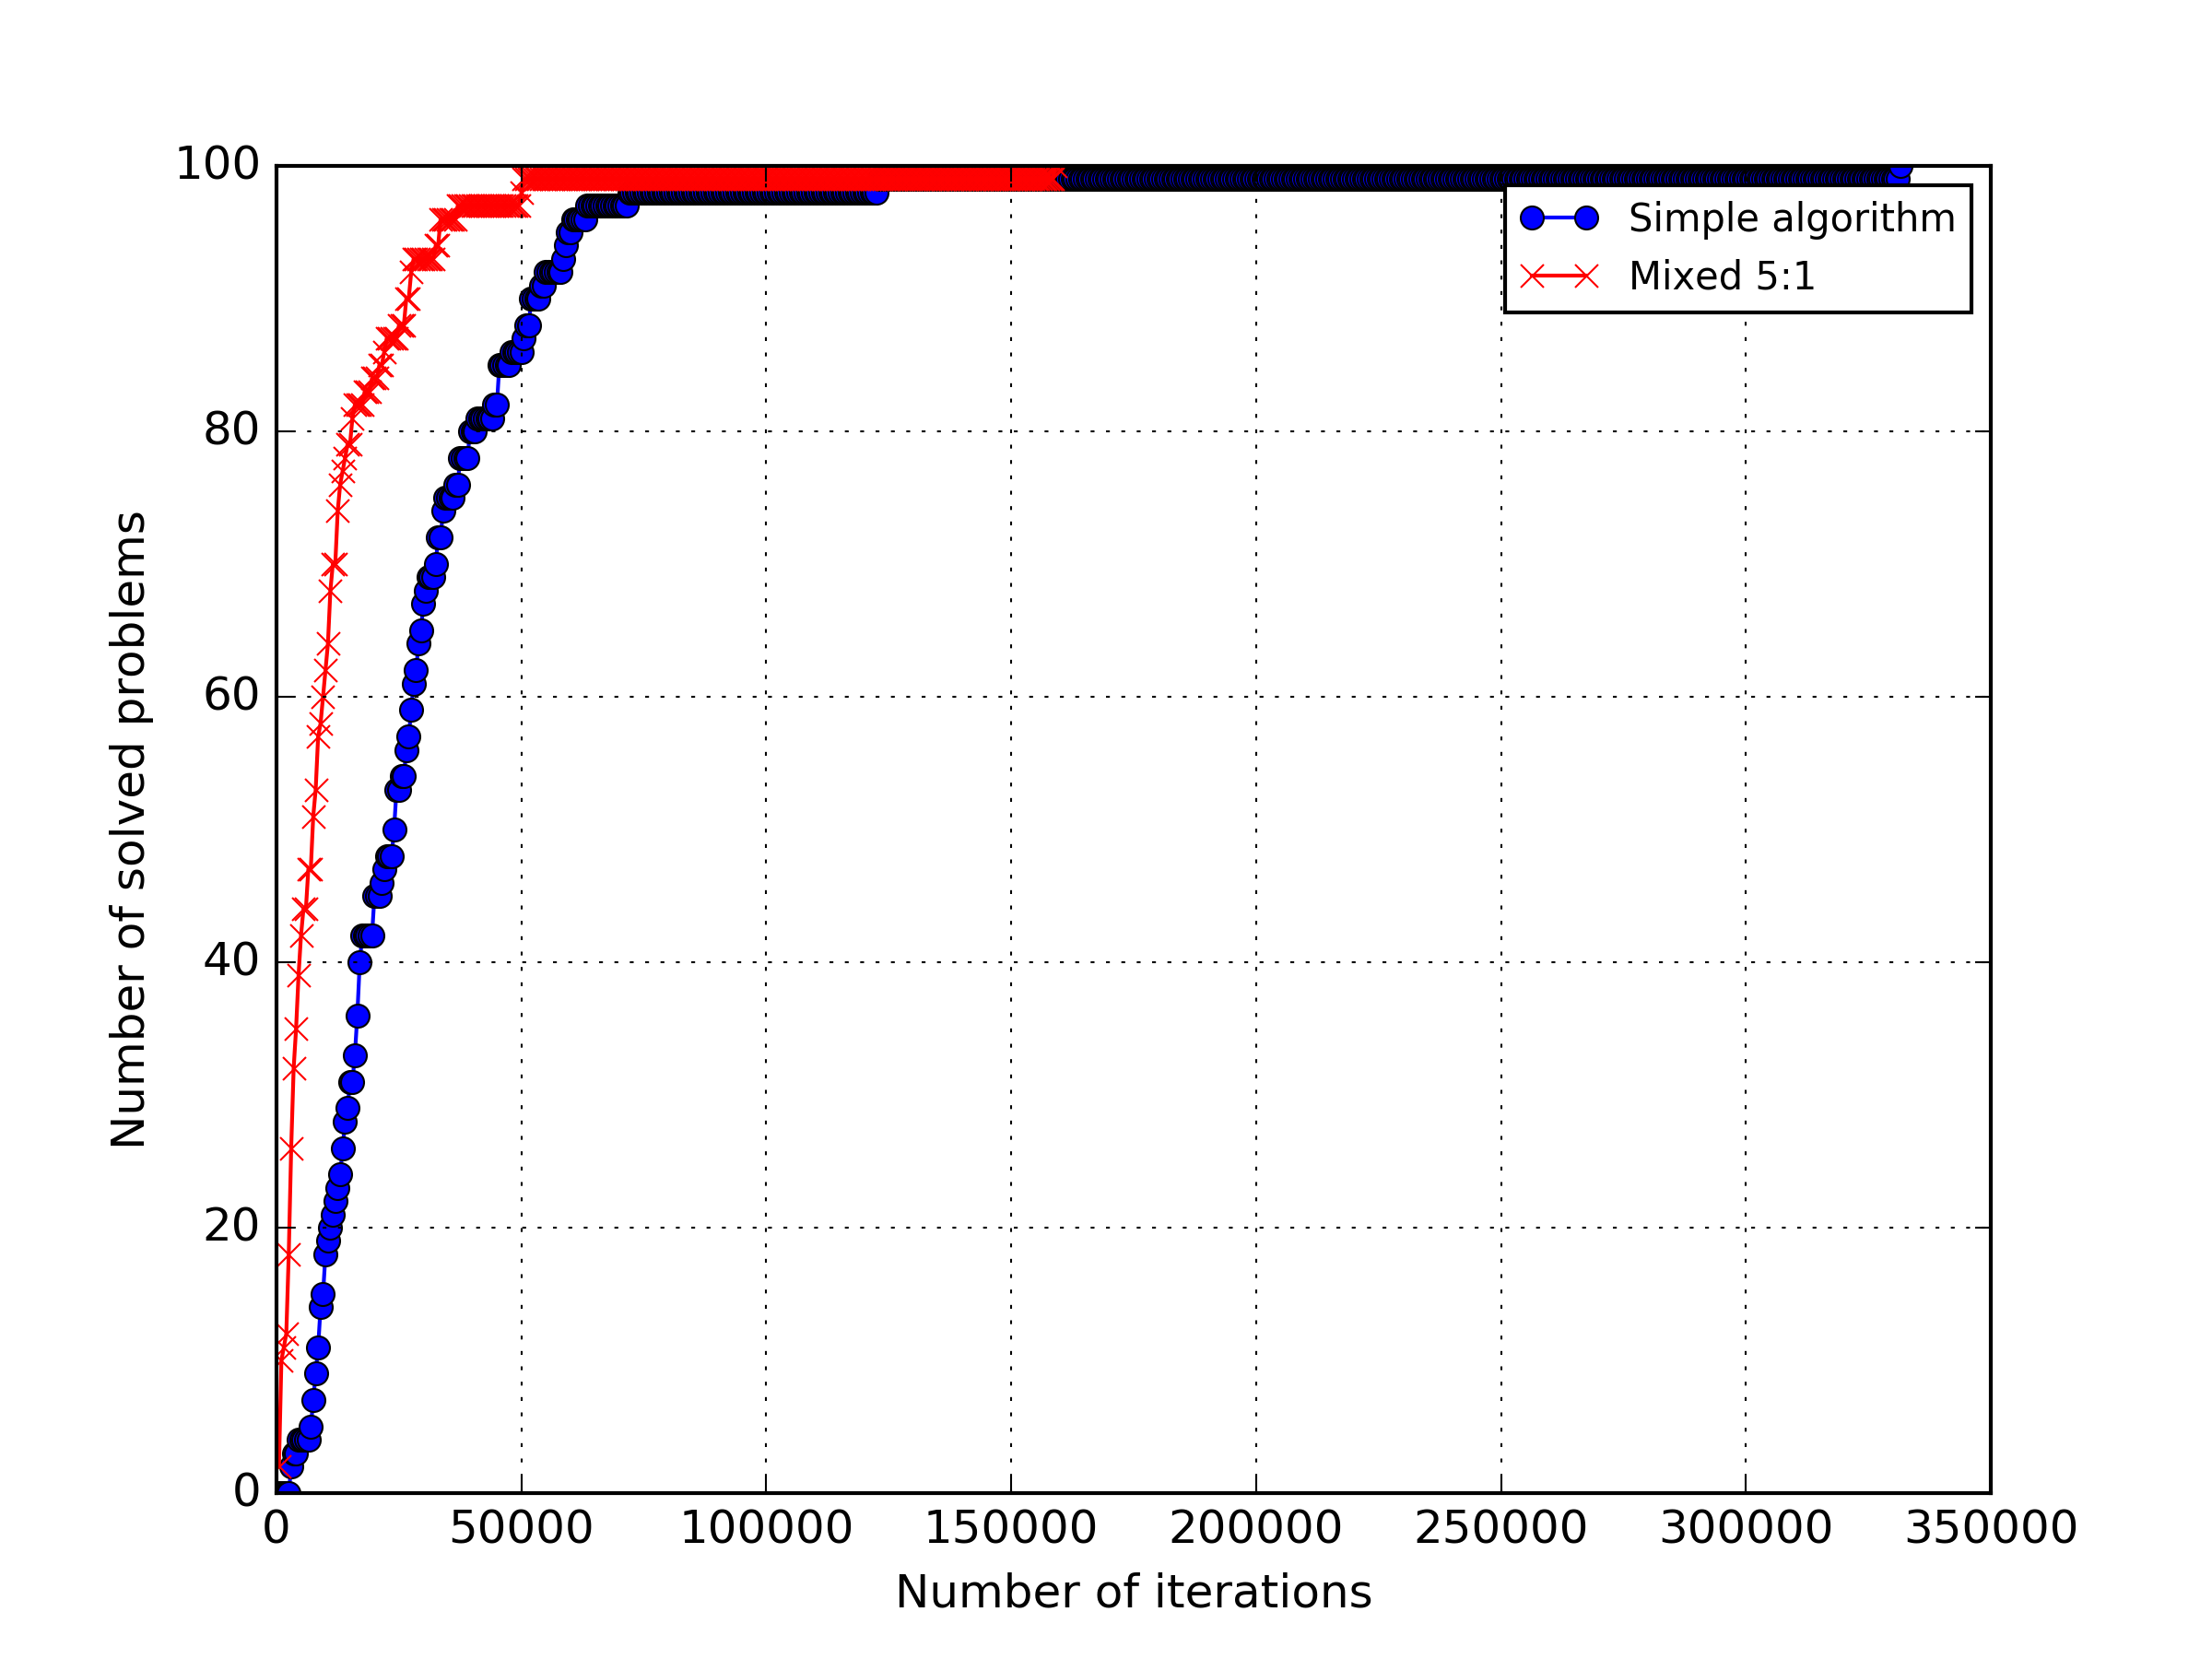
\includegraphics[width=0.75\textwidth]{pictures/mixed_op4d.png}
  \caption{Операционные характеристики обычного и смешанного АГП на классе GKLS 4d Simple}
  \label{fig:localMixOP4d}
\end{figure}
\par
Из-за того, что интервал имеет сразу две характеристики, появляется проблема эффективной реализации смешанного алгоритма. Если интервал имеет одну характеристику, то для выбора максимальной
достаточно организовать приоритетную очередь характеристик.
Причём перезаполнение такой очереди необходимо не на каждой итерации: в большинстве случаев характеристики интервалов не меняются, достаточно удалить разбиваемый интервал и вставить в очередь два новых.
Такая организация работы метода позволяет существенно сократить объём вычислений. При наличии у интервала двух характеристик можно организовать две связанные очереди. В этом случае необходимо предусмотреть
процедуру синхронизации двух очередей.
\par
Перечислим операции, при которых необходима синхронизаия:
\begin{itemize}
  \item вставка интервала сразу в обе очереди;
  \item удаление интервала из какой-либо очереди.
  %\item восстановление внутренней структуры очереди после модификации связанной очереди.
\end{itemize}
\par
Синхронизация достигается путём введения перекрёстных ссылок между элементами очередей. На рис. \ref{fig:heaps} приведена схема связанных очередей. Элемент очереди представляет собой
совокупность ключа (\textbf{LocalR} или \textbf{R}), указателя на интервал (\textbf{pInterval}) и указателя на элемент связанной очереди, соответствующий тому же интервалу (\textbf{pLinkedElement}).
Опишем подробнее алгоритмы вставки и удаления элементов.
\par
Вставка элемента в пару связанных очередей.
\begin{enumerate}
  \item Попытаться вставить элемент в очередь глобальных характеристик (он может быть не вставлен, если имеет слишком низкий приоритет).
  \item Попытаться вставить элемент в очередь локальных характеристик (он может быть не вставлен, если имеет слишком низкий приоритет).
  \item Если элемент интервал вставлен в обе очереди, то выставить перекрёстные ссылки.
\end{enumerate}
\par
Удаление элемента с минимальным ключом:
\begin{enumerate}
  \item Удалить элемент с минимальным ключом из очереди, запомнить указатель \textbf{pLinkedElement}.
  \item Если \textbf{pLinkedElement} ненулевой, то вызвать процедуру удаления элемента, на который указывает \textbf{pLinkedElement} в структуре данных, хранящей связянную очередь.
\end{enumerate}
\par
Последний момент, который надо учесть при реализации: вставка или удаление элемента очереди приводит к тому, что необходимо восстановить её внутреннюю структуру.
Если очередь хранится в куче, то восстанавливается свойство кучеобразности. Во время этого процесса
требуется производить попарные перестановки элементов, а значит, необходимо обновлять ссылки на эти элементы в связанной очереди.
\begin{figure}[ht]
	\center
  \includegraphics[width=0.9\textwidth]{pictures/examin_heaps.png}
  \caption{Схема устройства связянных очередей}
  \label{fig:heaps}
\end{figure}
\par
Стоит заметить, что внесённые модификации (в основном эта работа со ссылками) не увеличивают ассимптотическую сложность выполнения операций вставки и удаления по сравнению с единственной очередью.

\section{Заключение}
В ходе работы были получены следующие практические результаты:
\begin{itemize}
  \item реализован метод локальной оптимизации Хука-Дживса (код в приложении \ref{attach1});
  \item в системе ExaMin реализованы различные стратегии использования локального поиска;
  \item в рамках ExaMin реализована поддержка смешанного алгоритма глобального поиска, а также эффективные структуры данных, необходимые для этого алгоритма (фрагменты кода в приложении \ref{attach2})
  \item был проведён отдельный эксперимент для выяснения возможности практического использования многоуровневых развёрток.
\end{itemize}


\newpage
%\nocite{*}
\addcontentsline{toc}{section}{Список литературы}
\printbibliography
\newpage
\section{Приложения}
\subsection{Приложение 1}
\label{attach1}

\begin{lstlisting}[frame=single]
#ifndef __LOCALMETHOD_H__
#define __LOCALMETHOD_H__

#include "parameters.h"
#include "task.h"
#include "data.h"
#include "common.h"
#include <vector>

#define MAX_LOCAL_TRIALS_NUMBER 10000

class TLocalMethod
{
protected:

	int mDimension;
	int mConstraintsNumber;
	int mTrialsCounter;
	int mMaxTrial;

	TTrial mBestPoint;
	std::vector<TTrial> mSearchSequence;
	TTask* mPTask;

	bool mIsLogPoints;

	double mEps;
	double mStep;
	double mStepMultiplier;

	OBJECTIV_TYPE *mFunctionsArgument;
	OBJECTIV_TYPE *mStartPoint;
	OBJECTIV_TYPE* mCurrentPoint;
	OBJECTIV_TYPE* mCurrentResearchDirection;
	OBJECTIV_TYPE* mPreviousResearchDirection;

	double MakeResearch(OBJECTIV_TYPE*);
	void DoStep();
	double EvaluateObjectiveFunctiuon(const OBJECTIV_TYPE*);

public:

	TLocalMethod();
	TLocalMethod(TParameters _params, TTask* _pTask, TTrial _startPoint, bool logPoints = false);
	~TLocalMethod();

	void SetEps(double);
	void SetInitialStep(double);
	void SetStepMultiplier(double);
	void SetMaxTrials(int);

	int GetTrialsCounter() const;
	std::vector<TTrial> GetSearchSequence() const;

	TTrial StartOptimization();
};

#endif //__LOCALMETHOD_H__
\end{lstlisting}
\begin{lstlisting}[frame=single]
#include "local_method.h"
#include <cmath>
#include <cstring>
#include <algorithm>

TLocalMethod::TLocalMethod(TParameters _params, TTask* _pTask, TTrial _startPoint, bool logPoints)
{
	mEps = _params.Epsilon / 100;
	if (mEps > 0.0001)
		mEps = 0.0001;
	mBestPoint = _startPoint;
	mStep = _params.Epsilon * 2;
	mStepMultiplier = 2;
	mTrialsCounter = 0;
	mIsLogPoints = logPoints;

	mPTask = _pTask;

	mDimension = mPTask->GetN() - mPTask->GetFixedN();
	mConstraintsNumber = mPTask->GetNumOfFunc() - 1;

	mStartPoint = new OBJECTIV_TYPE[mDimension];
	std::memcpy(mStartPoint,
		_startPoint.y + mPTask->GetFixedN(),
		mDimension * sizeof(OBJECTIV_TYPE));

	mFunctionsArgument = new OBJECTIV_TYPE[mPTask->GetN()];
	std::memcpy(mFunctionsArgument,
		_startPoint.y,
		mPTask->GetN() * sizeof(OBJECTIV_TYPE));
	mMaxTrial = MAX_LOCAL_TRIALS_NUMBER;
}

TLocalMethod::TLocalMethod() : mPTask(NULL), mStartPoint(NULL),
mFunctionsArgument(NULL), mMaxTrial(MAX_LOCAL_TRIALS_NUMBER)
{
}

TLocalMethod::~TLocalMethod()
{
	if (mStartPoint)
		delete[] mStartPoint;
	if (mFunctionsArgument)
		delete[] mFunctionsArgument;
}

void TLocalMethod::DoStep()
{
	for (int i = 0; i < mDimension; i++)
		mCurrentPoint[i] = (1 + mStepMultiplier)*mCurrentResearchDirection[i] -
		mStepMultiplier*mPreviousResearchDirection[i];
}

TTrial TLocalMethod::StartOptimization()
{
	int k = 0, i = 0;
	bool needRestart = true;
	double currentFValue, nextFValue;
	mTrialsCounter = 0;

	mCurrentPoint = new OBJECTIV_TYPE[mDimension];
	mCurrentResearchDirection = new OBJECTIV_TYPE[mDimension];
	mPreviousResearchDirection = new OBJECTIV_TYPE[mDimension];

	while (mTrialsCounter < mMaxTrial) {
		i++;
		if (needRestart) {
			k = 0;
			std::memcpy(mCurrentPoint, mStartPoint, sizeof(OBJECTIV_TYPE)*mDimension);
			std::memcpy(mCurrentResearchDirection, mStartPoint, sizeof(OBJECTIV_TYPE)*mDimension);
			currentFValue = EvaluateObjectiveFunctiuon(mCurrentPoint);
			needRestart = false;
		}

		std::swap(mPreviousResearchDirection, mCurrentResearchDirection);
		std::memcpy(mCurrentResearchDirection, mCurrentPoint, sizeof(OBJECTIV_TYPE)*mDimension);
		nextFValue = MakeResearch(mCurrentResearchDirection);

		if (currentFValue > nextFValue) {
			DoStep();

			if (mIsLogPoints)
			{
				TTrial currentTrial;
				currentTrial.index = mBestPoint.index;
				currentTrial.FuncValues[currentTrial.index] = nextFValue;
				std::memcpy(currentTrial.y, mFunctionsArgument, sizeof(OBJECTIV_TYPE)*mPTask->GetFixedN());
				std::memcpy(currentTrial.y + mPTask->GetFixedN(), mCurrentPoint, sizeof(OBJECTIV_TYPE)*mDimension);
				mSearchSequence.push_back(currentTrial);
			}
			k++;
			currentFValue = nextFValue;
		}
		else if (mStep > mEps) {
			if (k != 0)
				std::memcpy(mStartPoint, mPreviousResearchDirection, sizeof(OBJECTIV_TYPE)*mDimension);
			else
				mStep /= mStepMultiplier;
			needRestart = true;
		}
		else
			break;
	}

	if (currentFValue < mBestPoint.FuncValues[mConstraintsNumber])
	{
		std::memcpy(mBestPoint.y + mPTask->GetFixedN(),
			mPreviousResearchDirection, sizeof(OBJECTIV_TYPE)*mDimension);
		mBestPoint.FuncValues[mConstraintsNumber] = currentFValue;
		mSearchSequence.push_back(mBestPoint);
	}

	delete[] mCurrentPoint;
	delete[] mPreviousResearchDirection;
	delete[] mCurrentResearchDirection;

	return mBestPoint;
}

double TLocalMethod::EvaluateObjectiveFunctiuon(const OBJECTIV_TYPE* x)
{
	if (mTrialsCounter >= mMaxTrial)
		return HUGE_VAL;

	for (int i = 0; i < mDimension; i++)
		if (x[i] < mPTask->GetA()[mPTask->GetFixedN() + i] ||
			x[i] > mPTask->GetB()[mPTask->GetFixedN() + i])
			return HUGE_VAL;

	std::memcpy(mFunctionsArgument + mPTask->GetFixedN(), x, mDimension * sizeof(OBJECTIV_TYPE));
	for (int i = 0; i <= mConstraintsNumber; i++)
	{
		double value = mPTask->GetFuncs()[i](mFunctionsArgument);
		if (i < mConstraintsNumber && value > 0)
		{
			mTrialsCounter++;
			return HUGE_VAL;
		}
		else if (i == mConstraintsNumber)
		{
			mTrialsCounter++;
			return value;
		}
	}

	return HUGE_VAL;
}

void TLocalMethod::SetEps(double eps)
{
	mEps = eps;
}

void TLocalMethod::SetInitialStep(double value)
{
	mStep = value;
}

void TLocalMethod::SetStepMultiplier(double value)
{
	mStepMultiplier = value;
}

void TLocalMethod::SetMaxTrials(int count)
{
	mMaxTrial = std::min(count, MAX_LOCAL_TRIALS_NUMBER);
}

int TLocalMethod::GetTrialsCounter() const
{
	return mTrialsCounter;
}

std::vector<TTrial> TLocalMethod::GetSearchSequence() const
{
	return mSearchSequence;
}

double TLocalMethod::MakeResearch(OBJECTIV_TYPE* startPoint)
{
	double bestValue = EvaluateObjectiveFunctiuon(startPoint);

	for (int i = 0; i < mDimension; i++)
	{
		startPoint[i] += mStep;
		double rightFvalue = EvaluateObjectiveFunctiuon(startPoint);

		if (rightFvalue > bestValue)
		{
			startPoint[i] -= 2 * mStep;
			double leftFValue = EvaluateObjectiveFunctiuon(startPoint);
			if (leftFValue > bestValue)
				startPoint[i] += mStep;
			else
				bestValue = leftFValue;
		}
		else
			bestValue = rightFvalue;
	}

	return bestValue;
}
\end{lstlisting}

\subsection{Приложение 2}
\label{attach2}
\begin{lstlisting}[frame=single]
#ifndef __DUAL_QUEUE_H__
#define __DUAL_QUEUE_H__

#include "minmaxheap.h"
#include "common.h"
#include "queue_common.h"

class TPriorityDualQueue : public TPriorityQueueCommon
{
protected:
	int MaxSize;
	int CurLocalSize;
	int CurGlobalSize;

	MinMaxHeap< TQueueElement, _less >* pGlobalHeap;
	MinMaxHeap< TQueueElement, _less >* pLocalHeap;

	void DeleteMinLocalElem();
	void DeleteMinGlobalElem();
	void ClearLocal();
	void ClearGlobal();
public:

	TPriorityDualQueue(int _MaxSize = DefaultQueueSize); // _MaxSize must be qual to 2^k - 1
	~TPriorityDualQueue();

	int GetLocalSize() const;
	int GetSize() const;
	int GetMaxSize() const;
	bool IsLocalEmpty() const;
	bool IsLocalFull() const;
	bool IsEmpty() const;
	bool IsFull() const;

	void Push(double globalKey, double localKey, void *value);
	void PushWithPriority(double globalKey, double localKey, void *value);
	void Pop(double *key, void **value);

	void PopFromLocal(double *key, void **value);

	void Clear();
	void Resize(int size);
};
#endif
\end{lstlisting}

\begin{lstlisting}[frame=single]
#include "dual_queue.h"

TPriorityDualQueue::TPriorityDualQueue(int _MaxSize)
{
	MaxSize = _MaxSize;
	CurGlobalSize = CurLocalSize = 0;
	pLocalHeap = new MinMaxHeap< TQueueElement, _less >(MaxSize);
	pGlobalHeap = new MinMaxHeap< TQueueElement, _less >(MaxSize);
}

TPriorityDualQueue::~TPriorityDualQueue()
{
	delete pLocalHeap;
	delete pGlobalHeap;
}

void TPriorityDualQueue::DeleteMinLocalElem()
{
	TQueueElement tmp = pLocalHeap->popMin();
	CurLocalSize--;

	//update linked element in the global queue
	if (tmp.pLinkedElement != NULL)
		tmp.pLinkedElement->pLinkedElement = NULL;
}

void TPriorityDualQueue::DeleteMinGlobalElem()
{
	TQueueElement tmp = pGlobalHeap->popMin();
	CurGlobalSize--;

	//update linked element in the local queue
	if (tmp.pLinkedElement != NULL)
		tmp.pLinkedElement->pLinkedElement = NULL;
}

int TPriorityDualQueue::GetLocalSize() const
{
	return CurLocalSize;
}

int TPriorityDualQueue::GetSize() const
{
	return CurGlobalSize;
}

int TPriorityDualQueue::GetMaxSize() const
{
	return MaxSize;
}

bool TPriorityDualQueue::IsLocalEmpty() const
{
	return CurLocalSize == 0;
}

bool TPriorityDualQueue::IsLocalFull() const
{
	return CurLocalSize == MaxSize;
}

bool TPriorityDualQueue::IsEmpty() const
{
	return CurGlobalSize == 0;
}

bool TPriorityDualQueue::IsFull() const
{
	return CurGlobalSize == MaxSize;
}

void TPriorityDualQueue::Push(double globalKey, double localKey, void * value)
{
	TQueueElement* pGlobalElem = NULL, *pLocalElem = NULL;
	//push to a global queue
	if (!IsFull()) {
		CurGlobalSize++;
		pGlobalElem = pGlobalHeap->push(TQueueElement(globalKey, value));
	}
	else {
		if (globalKey > pGlobalHeap->findMin().Key) {
			DeleteMinGlobalElem();
			CurGlobalSize++;
			pGlobalElem = pGlobalHeap->push(TQueueElement(globalKey, value));
		}
	}
	//push to a local queue
	if (!IsLocalFull()) {
		CurLocalSize++;
		pLocalElem = pLocalHeap->push(TQueueElement(localKey, value));
	}
	else {
		if (localKey > pLocalHeap->findMin().Key) {
			DeleteMinLocalElem();
			CurLocalSize++;
			pLocalElem = pLocalHeap->push(TQueueElement(localKey, value));
		}
	}
	//link elements
	if (pGlobalElem != NULL && pLocalElem != NULL) {
		pGlobalElem->pLinkedElement = pLocalElem;
		pLocalElem->pLinkedElement = pGlobalElem;
	}
}

void TPriorityDualQueue::PushWithPriority(double globalKey, double localKey, void * value)
{
	TQueueElement* pGlobalElem = NULL, *pLocalElem = NULL;
	//push to a global queue
	if (!IsEmpty()) {
		if (globalKey > pGlobalHeap->findMin().Key) {
			if (IsFull())
				DeleteMinGlobalElem();
			CurGlobalSize++;
			pGlobalElem = pGlobalHeap->push(TQueueElement(globalKey, value));
		}
	}
	else {
		CurGlobalSize++;
		pGlobalElem = pGlobalHeap->push(TQueueElement(globalKey, value));
	}
	//push to a local queue
	if (!IsLocalEmpty()) {
		if (localKey > pLocalHeap->findMin().Key) {
			if (IsLocalFull())
				DeleteMinLocalElem();
			CurLocalSize++;
			pLocalElem = pLocalHeap->push(TQueueElement(localKey, value));
		}
	}
	else {
		CurLocalSize++;
		pLocalElem = pLocalHeap->push(TQueueElement(localKey, value));
	}
	//link elements
	if (pGlobalElem != NULL && pLocalElem != NULL) {
		pGlobalElem->pLinkedElement = pLocalElem;
		pLocalElem->pLinkedElement = pGlobalElem;
	}
}

void TPriorityDualQueue::PopFromLocal(double * key, void ** value)
{
	TQueueElement tmp = pLocalHeap->popMax();
	*key = tmp.Key;
	*value = tmp.pValue;
	CurLocalSize--;

	//delete linked element from the global queue
	if (tmp.pLinkedElement != NULL) {
		pGlobalHeap->deleteElement(tmp.pLinkedElement);
		CurGlobalSize--;
	}
}

void TPriorityDualQueue::Pop(double * key, void ** value)
{
	TQueueElement tmp = pGlobalHeap->popMax();
	*key = tmp.Key;
	*value = tmp.pValue;
	CurGlobalSize--;

	//delete linked element from the local queue
	if (tmp.pLinkedElement != NULL)	{
		pLocalHeap->deleteElement(tmp.pLinkedElement);
		CurLocalSize--;
	}
}

void TPriorityDualQueue::Clear()
{
	ClearLocal();
	ClearGlobal();
}

void TPriorityDualQueue::Resize(int size)
{
	MaxSize = size;
	CurGlobalSize = CurLocalSize = 0;
	delete pLocalHeap;
	delete pGlobalHeap;
	pLocalHeap = new MinMaxHeap< TQueueElement, _less >(MaxSize);
	pGlobalHeap = new MinMaxHeap< TQueueElement, _less >(MaxSize);
}

void TPriorityDualQueue::ClearLocal()
{
	pLocalHeap->clear();
	CurLocalSize = 0;
}

void TPriorityDualQueue::ClearGlobal()
{
	pGlobalHeap->clear();
	CurGlobalSize = 0;
}
\end{lstlisting}


\endgroup

\end{document}
